%!TEX TS-program = xelatex
\documentclass[a4paper]{article}  

\usepackage{setspace}%Пакет с интервалами

%Работа с цитатами

\usepackage[font={small,it}]{caption}
\usepackage{float} % пакеты с графикой
\usepackage{tikz}
\usepackage{pgfplots}
\usepackage{matlab-prettifier,graphics,epstopdf}
\usepackage{pstool}
\usepackage{siunitx}
\pgfplotsset{compat=1.9}

\usepackage[english,russian]{babel} %языковые пакеты
%\usepackage{mathtext,amsmath,unicode-math,empheq}
\usepackage{amsmath,unicode-math,empheq} %на линуксе нет mathtext

\usepackage[utf8]{inputenc}%кодировка шрифта utf-8
\usepackage{fontenc} %шрифты
\usepackage{fontspec}

\usepackage{multicol}%Мультиколонки
\setlength{\columnsep}{1cm}

%Шрифты в заголовках
\usepackage{titlesec}
\usepackage{secdot}
\titleformat{\section}
{\centering\normalfont\fontsize{14}{21}\bfseries}{\thesection.}{1em}{}
\titleformat{\subsection}
{\centering\normalfont\fontsize{14}{21}\bfseries}{\thesubsection.}{1em}{}
\titleformat{\subsubsection}
{\centering\normalfont\fontsize{14}{21}\bfseries}{\thesubsubsection.}{1em}{}
%\titlelabel{\thetitle .\quad}
%

\usepackage{cancel}%зачеркивания в формулах
%\usepackage{icomma}%умная запятая
\usepackage[bookmarks=true, colorlinks=true,unicode=true,urlcolor=black,linkcolor=black, anchorcolor=black,citecolor=black,menucolor=black, filecolor=black]{hyperref}%гиперссылки

\usepackage[includeheadfoot=true]{geometry}%параметры страницы
\geometry{a4paper, total={170mm,257mm},left=30mm,right=15mm,top=20mm,bottom=20mm}
\usepackage{indentfirst} %делать отступ в начале параграфа
\setlength{\parindent}{7.4mm} %7,4мм

\numberwithin{equation}{section} %нумерация уравнений с номерами разделов
\renewcommand{\refname}{Список источников} %Вместо "Список литературы" будет "Список источников"
\usepackage{csquotes}
\bibliographystyle{gost-numeric}
%\usepackage[backend=biber,bibencoding=utf8,style=numeric-comp,bibstyle=gost-numeric]{biblatex}
\usepackage[parentracker=true,backend=biber,bibencoding=utf8,citestyle=gost-numeric,bibstyle=gost-numeric]{biblatex}
%\addbibresource{biblio.bib}
\addbibresource{Collection.bib}

%\singlespacing
%\onehalfspacing%полуторный интервал
%\doublespacing
\setmainfont{Times New Roman}%тут всё просто)

\usepackage{xparse}

\let\oldsection\section
\makeatletter
\newcounter{@secnumdepth}
\RenewDocumentCommand{\section}{s o m}{%
	\IfBooleanTF{#1}
	{\setcounter{@secnumdepth}{\value{secnumdepth}}% Store secnumdepth
		\setcounter{secnumdepth}{0}% Print only up to \chapter numbers
		\oldsection{#3}% \section*
		\setcounter{secnumdepth}{\value{@secnumdepth}}}% Restore secnumdepth
	{\IfValueTF{#2}% \section
		{\oldsection[#2]{#3}}% \section[.]{..}
		{\oldsection{#3}}}% \section{..}
}
\makeatother
% подгрузить преамбулу
\begin{document}
\fontsize{14}{21pt}\selectfont	
\setcounter{page}{2}
\tableofcontents
\newpage

\section*{Введение}
	
Изучение ионизированных структур, в том числе, плазмы, в отдельности, является одним из приоритетных направлений в области как теоретической, так и прикладной физики. Особенную роль играет способность подобных структур к генерации электромагнитных волн под внешним воздействием. С учетом того, что изучаемая в таких случаях плазма по факту представляет из себя сильно ионизированный газ, под внешним воздействием обычно понимают электромагнитное поле разной формы, структуры, и способа генерации, хотя чаще всего в прикладных исследованиях и экспериментах используют именно лазерную генерацию. Таким образом конструируются и моделируются лазерно-плазменные излучатели.

В данной работе численно исследуется группа однотипных частных случаев такой генерации, когда в некий определенный, далее называемый начальным моментом, бесконечно малый (узкий) промежуток времени в плазме заданной формы и структуры возбуждается ток, после чего задачей исследователя является изучение того, как данная система будет себя вести в дальнейшем во времени и пространстве. То есть одной из главных задач в подобных работах, в том числе и этой, является получение и изучение пространственно временной эволюции магнитных и электрических полей, а также аналогичного распределения (эволюции) тока. После этого с полученными данными уже можно работать производя дальнейшие известные и, впрочем, стандартные преобразования, такие как, получение спектральных характеристик, нахождение энергетических зависимостей и так далее. Впрочем, на точность и правдоподобность уже этих данных будет влиять качество и точность построенного пространственно временного распределения, что отчасти имеет отражение и в данной работе.

Данная работа фактически является продолжением и модификацией задачи о моделировании плазменного цилиндрического излучателя. Однако в данной задаче дополнительно добавляется и учитывается новое явление касательно распространения ионизации внутри самого излучателя. То есть мы фактически снимаем одну из идеализаций в постановке задачи и делаем последнюю более приближенной к реальным исследуемым моделям.

Для изучения поставленного вопроса -- как и в предыдущий раз -- требуется не столько вычислительная мощность, сколько корректно настроенный алгоритм, на входе которого <<подаются>> определенные параметры поставленной задачи, а на выводе получаются требуемые к нахождению данные, причем они должны быть согласованы с теорией и если отличаться от неё, то на очень малую величину. Основной задачей данной работы является создание такого алгоритма в виде вычислительного кода. Поставлена задача создания такого вычислительного кода для решения точных уравнений Максвелла применимо к заданной системе, описанной ниже.

\newpage
\section{Постановка задачи и основные соотношения}
\subsection{Постановка задачи}

Пусть дан цилиндр радиуса $R_{2}$, бесконечный вдоль своей оси (оси $z$), заполненный газом. Пусть вдоль оси $z$ в начальный момент времени попадает ультракороткий лазерный импульс такой конфигурации, что данный газ мгновенно ионизируется в точке <<попадания>> импульса и эта ионизация начинает распространятся по $z$ с заданной скоростью $V$, называемой <<бегучестью плазмы>>. Ионизация порождает бегущий ионизационный фронт остаточного тока и заданной концентрации заряженных частиц в плазме. Причём эта концентрация равномерно распределена по сечению цилиндра и имеет заданное симметричное -- не зависящее от полярного угла -- пространственное распределение по радиусу цилиндра. От его оси при $r=0$ до определенного радиуса $R_{1}=const$ плазменная концентрация равна определенному заданному значению $N_{0}$, далее от $R_{1}$ до $R_{2}$ плавно спадает до нуля, после чего, соответственно, переходит в вакуум.

Обозначим такой закон спадания концентрации в сечении цилиндра как некую заданную функцию $f(r)$:
\begin{equation}
	f(r)=
	\begin{cases}
		1, & r<R_{1}\\
		\cos^{2}\left(\frac{\pi(r-R_{1})}{2(R_{2}-R_{1})}\right), & R_{1}<r<R_{2}\\
		0, & r>R_{2}
	\end{cases}			
	\label{eq:f(r)}
\end{equation}

Концентрация и плазменная частота равны соответственно:
\begin{align}
	N(r)=N_{0}f(r)\label{eq:N(r)}\\
	\omega_p^2 = \omega_{p0}^{2} f(r)
	\label{eq:omega_p(r)}
\end{align}
\newpage
Распределение плазменной концентрации \eqref{eq:N(r)} в таком случае имеет вид:
\begin{figure}[H]
	\begin{tikzpicture}
		\begin{axis}[
			xlabel = {\large{$r$}},
			ylabel = {\large{$N(r)$}},
			major grid style = {dashed,black, line width=1pt},
			grid = major,
			axis lines=middle,
			xtick={0.0467,0.1085}, 
			xticklabels={\large{$R_{1}$},\large{$R_{2}$}},
			ytick={0,1},
			yticklabels={\large{0},\large{$N_{0}$}},
			%minor tick num=1,					
			table/col sep = semicolon,
			height = 0.3\paperheight, 
			width = 0.75\paperwidth,
			%xmin = 0.002,
			%xmax = 0.2,
			ymin=0,
			ymax=1.2,
			/pgf/number format/1000 sep={}
			]			
			\addplot+[color=black,line width=2.5pt,mark=none] table [x={r},y={fr}] {fr.csv}; 	
			%\draw[->] (0,0) -- (2,0); % Ох			 	
		\end{axis}		 			
	\end{tikzpicture}
	\caption{Распределение плазменной концентрации в зависимости от $r$.}
	\label{ris:f(r)}
\end{figure}




А сечение цилиндра схематично представлено на рис.\ref{pic:cill}
\begin{figure}[H]
	\begin{center}
		\begin{tikzpicture}[x=0.75pt,y=0.75pt,yscale=-1,xscale=1]
	%uncomment if require: \path (0,575); %set diagram left start at 0, and has height of 575
	
	%Shape: Circle [id:dp9505457780936883] 
	\draw   (198,336) .. controls (198,257.58) and (261.58,194) .. (340,194) .. controls (418.42,194) and (482,257.58) .. (482,336) .. controls (482,414.42) and (418.42,478) .. (340,478) .. controls (261.58,478) and (198,414.42) .. (198,336) -- cycle ;
	%Shape: Circle [id:dp6651156438339156] 
	\draw  [dash pattern={on 4.5pt off 4.5pt}] (227.75,336) .. controls (227.75,274.01) and (278.01,223.75) .. (340,223.75) .. controls (401.99,223.75) and (452.25,274.01) .. (452.25,336) .. controls (452.25,397.99) and (401.99,448.25) .. (340,448.25) .. controls (278.01,448.25) and (227.75,397.99) .. (227.75,336) -- cycle ;
	%Straight Lines [id:da3498014946233359] 
	\draw  [dash pattern={on 4.5pt off 4.5pt}]  (340,336) -- (452.25,336) ;
	%Straight Lines [id:da5645909598159475] 
	\draw    (268,213) -- (340,336) ;
	
	% Text Node
	\draw (395.5,332) node [anchor=south] [inner sep=0.75pt]   [align=left] {\large{$R_{1}$}};
	% Text Node
	\draw (312,268) node [anchor=north west][inner sep=0.75pt]   [align=left] {\large{$R_{2}$}};
	
	
\end{tikzpicture}
	\end{center}		
	\caption{Сечение цилиндра}
	\label{pic:cill}
\end{figure}

Положим что в начальный момент времени единовременно во всем пространстве цилиндра возбуждается ток с заданной плотностью (\ref{jt_0})
\begin{equation}
	\vec{j}|_{t=0}=j_0 f(r)\cdot\overrightarrow{x_0},\quad j_{0}=const
	\label{jt_0}
\end{equation}

При этом поля в начальный момент времени нулевые:
\begin{equation}
	\vec{E}|_{t=0}=0;\quad\vec{H}_{t=0}=0
\end{equation}

То есть ток возбуждается вдоль оси $x$, которая, в свою очередь, перпендикулярна оси цилиндра $z$. Данное распределение начального тока даёт нам возможность искать дальнейшее решение задачи в \textit{дипольном} виде, с заданной зависимостью от полярного угла, при этом подобная зависимость компонент полей и токов позволит нам значительно упростить решение задачи, сведя его к одномерному радиальному распределению искомых функций. 


\subsection{Основные соотношения}

Найдём выражение для плотности тока в плазме, используя известные соотношения \eqref{j:eNv} -- \eqref{eq:m_djdt}. Мы знаем определение плотности тока, как упорядоченного движения заряженных частиц. Пренебрегаем движением ионов в плазме по причине их много большей массы по сравнению с массой электронов. Будем считать что в изучаемой нами плазме движению подвержены только электроны.
\begin{equation}\label{j:eNv}
	\vec{j}=eN_{e}\vec{v}
\end{equation}
где $j$ -- искомая плотность тока, $e$ и $(N_{e}\equiv N)$ -- заряд электрона и концентрация электронов в плазме соответственно.
Продифференцируем \eqref{j:eNv}
один раз по времени
\begin{equation}\label{djdt}
	\frac{\partial \vec{j}}{\partial t}=eN\frac{\partial \vec{v}}{\partial t}
\end{equation}
а также запишем уравнение движения в электрическом поле плазменных частиц с учётом их соударений -- в таком случае вводится аналог силы трения
\begin{equation}\label{eq:dvizh}
	m\frac{\partial \vec{v}}{\partial t}=e\vec{E}-m\nu\vec{v}
\end{equation}
где $e$ -- модуль заряда электрона, $m$ -- масса электрона, $N$ -- концентрация электронов в плазме, $\nu$ -- частота соударений частиц.
Подставим \eqref{eq:dvizh} в \eqref{djdt}, предварительно разделив обе части уравнения \eqref{eq:dvizh} на $m$:
\begin{align}
	\frac{\partial\vec{j}}{\partial t}=eN\left(\frac{e}{m}\vec{E}-\nu\vec{v}\right)\\
	\frac{\partial\vec{j}}{\partial t}=\frac{e^{2}N}{m}\vec{E}-\nu eN\vec{v}\label{eq:m_djdt}
\end{align}
Используя \eqref{j:eNv} в \eqref{eq:m_djdt}, а также определение плазменной частоты \eqref{eq:omega_p0}
получаем окончательное уравнение для плотности тока в плазме:
\begin{equation}
	\frac{\partial\vec{j}}{\partial t}=\frac{\omega_{p}^{2}}{4\pi}\vec{E}-\nu\vec{j}
\end{equation}
где \begin{equation}\label{eq:omega_p0}
	\omega_{p}(r)=\sqrt{\frac{4\pi e^{2}N(r)}{m}}
\end{equation}

Записав уравнения Максвелла в дифференциальной форме в системе СГС вместе с уравнением \eqref{eq:omega_p0}:
\begin{equation}
	\left\{ 
	\begin{gathered}
		rot\vec{E}=-\cfrac{1}{c}\cfrac{\partial\vec{H}}{\partial t} \\
		rot\vec{H}=\cfrac{4\pi}{c}\vec{j}+\cfrac{1}{c}\cfrac{\partial\vec{E}}{\partial t} \\
		\dfrac{\partial\vec{j}}{\partial t}=\frac{{\omega_{p}}^{2}}{4\pi}\vec{E}-\nu\vec{j}
	\end{gathered}
	\right.		
	\label{eq:sys:start}
\end{equation}
мы получим основную фундаментальную систему уравнений, которую мы будем использовать для дальнейших расчетов в данной работе.

Используя \eqref{jt_0}, упростим систему \eqref{eq:sys:start}: так как искомая система представляет собой бесконечный цилиндр, проще всего будет искать решение в цилиндрической системе координат. Разложим начальный импульс \eqref{jt_0} по векторам не декартовой, а цилиндрической СК.

\begin{equation}
	{\vec {e}}_{x}=\cos \varphi {\vec {e}}_{\rho }-\sin \varphi {\vec {e}}_{\varphi }
\end{equation}

То есть:
\begin{equation}\label{x:to:cill}
	\vec{x}_{0}=\cos\varphi\cdot\vec{r}_{0}-\sin\varphi\cdot\vec{\varphi}_{0}
\end{equation}

Также распишем систему \eqref{eq:sys:start} в цилиндрической СК:

\begin{equation}\label{eq:maxwell_2}
	\begin{cases}
		\cfrac{1}{r}\cfrac{\partial E_{z}}{\partial\varphi}-\cfrac{\partial E_{\varphi}}{\partial z}=-\cfrac{1}{c}\cfrac{\partial H_{r}}{\partial t}\\
		\cfrac{\partial E_{r}}{\partial z}-\cfrac{\partial E_{z}}{\partial r}=-\cfrac{1}{c}\cfrac{\partial H_{\varphi}}{\partial t}\\
		\cfrac{1}{r}\left(\cfrac{\partial\left(rE_{\varphi}\right)}{\partial r}-\cfrac{\partial E_{r}}{\partial\varphi}\right)=-\cfrac{1}{c}\cfrac{\partial H_{z}}{\partial t}\\
		\cfrac{1}{r}\cfrac{\partial H_{z}}{\partial\varphi}-\cfrac{\partial H_{\varphi}}{\partial z}=\cfrac{4\pi}{c}j_{r}+\cfrac{1}{c}\cfrac{\partial E_{r}}{\partial t}\\
		\cfrac{\partial H_{r}}{\partial z}-\cfrac{\partial H_{z}}{\partial r}=\cfrac{4\pi}{c}j_{\varphi}+\cfrac{1}{c}\cfrac{\partial E_{\varphi}}{\partial t}\\
		\cfrac{1}{r}\left(\cfrac{\partial\left(rH_{\varphi}\right)}{\partial r}-\cfrac{\partial H_{r}}{\partial\varphi}\right)=\cfrac{4\pi}{c}j_{z}+\cfrac{1}{c}\cfrac{\partial E_{z}}{\partial t}\\
		\cfrac{\partial{j_{(r,\varphi,z)}}}{\partial t}=\cfrac{{\omega_{p}}^{2}}{4\pi}{E_{(r,\varphi,z)}}-\nu{j_{(r,\varphi,z)}}
	\end{cases}
\end{equation}


Воспользуемся методом разделения переменных, представим все исследуемые компоненты как произведение функции, зависящей только от времени и координаты на функцию, зависящей только от полярного угла.
\begin{equation}
	\begin{cases}
		j_{r}=j_{r}(r,t)\cos\varphi; &\quad j_{\varphi}=j_{\varphi}(r,t)\sin\varphi;\quad j_{z}=j_{z}(r,t)\cos\varphi;\\
		E_{r}=E_{r}(r,t)\cos\varphi; &\quad E_{\varphi}=E_{\varphi}(r,t)\sin\varphi;\quad E_{z}=E_{z}(r,t)\cos\varphi;\\
		H_{r}=H_{r}(r,t)\sin\varphi; &\quad H_{\varphi}=H_{\varphi}(r,t)\cos\varphi;\quad H_{z}=H_{z}(r,t)\sin\varphi;
	\end{cases}	
\label{eq:razdel_per}
\end{equation} 
\newpage
Получаем систему с так называемым \textit{дипольным} решением, с заданной зависимостью от угла, при этом сами исследуемые в дальнейшем компоненты в \eqref{eq:razdel_per} зависят только от времени, радиальной координаты, то есть от расстояния от оси цилиндра и координаты $z$. Учитывая то, что система уравнений \eqref{eq:maxwell_2} есть система уравнений в частных производных, подставив \eqref{eq:razdel_per} в \eqref{eq:maxwell_2}, получаем промежуточную систему уравнений:
\begin{equation}
	\begin{cases}		
		\cfrac{1}{r}E_{z}+\cfrac{\partial E_{\varphi}}{\partial z}=-\cfrac{1}{c}\cfrac{\partial H_{r}}{\partial t}\\
		\cfrac{\partial E_{r}}{\partial z}-\cfrac{\partial E_{z}}{\partial r}=-\cfrac{1}{c}\cfrac{\partial H_{\varphi}}{\partial t}\\
		\cfrac{1}{r}\left(\cfrac{\partial\left(rE_{\varphi}\right)}{\partial r}+E_{r}\right)=-\cfrac{1}{c}\cfrac{\partial H_{z}}{\partial t}\\
		\cfrac{1}{r}H_{z}-\cfrac{\partial H_{\varphi}}{\partial z}=\cfrac{4\pi}{c}j_{r}+\cfrac{1}{c}\cfrac{\partial E_{r}}{\partial t}\\
		\cfrac{\partial H_{r}}{\partial z}-\cfrac{\partial H_{z}}{\partial r}=\cfrac{4\pi}{c}j_{\varphi}+\cfrac{1}{c}\cfrac{\partial E_{\varphi}}{\partial t}\\
		\cfrac{1}{r}\left(\cfrac{\partial\left(rH_{\varphi}\right)}{\partial r}-H_{r}\right)=\cfrac{4\pi}{c}j_{z}+\cfrac{1}{c}\cfrac{\partial E_{z}}{\partial t}\\
		\cfrac{\partial{j_{(r,\varphi,z)}}}{\partial t}=\cfrac{{\omega_{p}}^{2}}{4\pi}{E_{(r,\varphi,z)}}-\nu{j_{(r,\varphi,z)}}
	\end{cases}
	\label{eq:maxwell_last}
\end{equation}

Для учета в системе уравнений бегучести плазмы введём новый параметр \\$\xi$ -- аналогичный времени $t$, и имеющий такую же размерность.
\begin{equation}
	\xi=t-\frac{z}{V}
	\label{eq:xi(t-z/V)}
\end{equation}

Где $V$ -- уже упомянутая бегучесть (скорость распространения ионизационного фронта). Производные по $z$ и по $t$ будут равны соответственно 
\begin{eqnarray}
	\cfrac{\partial}{\partial z} =& -\cfrac{1}{V}\cfrac{\partial}{\partial\xi}\\
	\cfrac{\partial}{\partial t} =& \cfrac{\partial}{\partial\xi}
\end{eqnarray}

Подставляя новые производные в \eqref{eq:maxwell_last}, получим:
\begin{equation}
	\begin{cases}		
		\cfrac{1}{r}E_{z}-\cfrac{1}{V}\cfrac{\partial E_{\varphi}}{\partial\xi}=-\cfrac{1}{c}\cfrac{\partial H_{r}}{\partial\xi}\\
		-\cfrac{1}{V}\cfrac{\partial E_{r}}{\partial\xi}-\cfrac{\partial E_{z}}{\partial r}=-\cfrac{1}{c}\cfrac{\partial H_{\varphi}}{\partial\xi}\\
		\cfrac{1}{r}\left(\cfrac{\partial\left(rE_{\varphi}\right)}{\partial r}+E_{r}\right)=-\cfrac{1}{c}\cfrac{\partial H_{z}}{\partial\xi}\\
		\cfrac{1}{r}H_{z}+\cfrac{1}{V}\cfrac{\partial H_{\varphi}}{\partial\xi}=\cfrac{4\pi}{c}j_{r}+\cfrac{1}{c}\cfrac{\partial E_{r}}{\partial\xi}\\
		-\cfrac{1}{V}\cfrac{\partial H_{r}}{\partial\xi}-\cfrac{\partial H_{z}}{\partial r}=\cfrac{4\pi}{c}j_{\varphi}+\cfrac{1}{c}\cfrac{\partial E_{\varphi}}{\partial\xi}\\
		\cfrac{1}{r}\left(\cfrac{\partial\left(rH_{\varphi}\right)}{\partial r}-H_{r}\right)=\cfrac{4\pi}{c}j_{z}+\cfrac{1}{c}\cfrac{\partial E_{z}}{\partial\xi}\\
		\cfrac{\partial{j_{(r,\varphi,z)}}}{\partial\xi}=\cfrac{{\omega_{p}}^{2}}{4\pi}{E_{(r,\varphi,z)}}-\nu{j_{(r,\varphi,z)}}
	\end{cases}
	\label{eq:last}
\end{equation}

Система \eqref{eq:last} содержит зависимости производных $H_{r}=H_{r}(E_{\varphi}); H_{\varphi}=H_{\varphi}(E_{r});\\E_{r}=E_{r}(H_{\varphi});E_{\varphi}=E_{\varphi}(H_{r}), $ однако окончательная система уравнений должна содержать только прямые зависимости от $r$ и $\xi$ для устранения <<перекрестных>> зависимостей последовательно выразим одну производную через другую и приведя подобные слагаемые, получаем окончательную систему:
\begin{equation}
	\begin{cases}
		\left(\cfrac{V^{2}c}{V^{2}-c^{2}}\right)\left(\cfrac{1}{r}H_{z}+\cfrac{c}{V}\cfrac{\partial E_{z}}{\partial r}-\cfrac{4\pi}{c}j_{r}\right)=\cfrac{\partial E_{r}}{\partial\xi}\\
		
		\left(\cfrac{V^{2}c}{V^{2}-c^{2}}\right)\left(-\cfrac{c}{V}\cfrac{1}{r}E_{z}-\cfrac{\partial H_{z}}{\partial r}-\cfrac{4\pi}{c}j_{\varphi}\right)=\cfrac{\partial E_{\varphi}}{\partial\xi}\\		
		
		\cfrac{c}{r}\left(\cfrac{\partial\left(r H_{\varphi}\right)}{\partial r}-H_{r}\right)-{4\pi}j_{z}=\cfrac{\partial E_{z}}{\partial\xi}\\
		
		\left(\cfrac{V^{2}c}{V^{2}-c^{2}}\right)\left(\cfrac{1}{r}E_{z}+\cfrac{c}{V}\left(\cfrac{\partial H_{z}}{\partial r}+\cfrac{4\pi}{c}j_{\varphi}\right)\right)=\cfrac{\partial H_{r}}{\partial\xi}\\
		
		\left(\cfrac{V^{2}c}{V^{2}-c^{2}}\right)\left(\cfrac{c}{V}\left(\cfrac{1}{r}H_{z}-\cfrac{4\pi}{c}j_{r}\right)+\cfrac{\partial E_{z}}{\partial r}\right)=\cfrac{\partial H_{\varphi}}{\partial\xi}\\
		
		-\cfrac{c}{r}\left(\cfrac{\partial\left(r E_{\varphi}\right)}{\partial r}+E_{r}\right)=\cfrac{\partial H_{z}}{\partial\xi}\\
		
		\cfrac{\partial j_{r,\varphi,z}}{\partial\xi}=\cfrac{\omega_{p}^{2}}{4\pi}E_{r,\varphi,z}-\nu j_{r,\varphi,z}
	\end{cases}		
	\label{eq:superlast}
\end{equation}

Для более наглядного и локального объяснения существования конечной скорости распространения ионизационного фронта можно перейти от базиса волновых скоростей к базису волновых чисел. По определению, фазовая скорость распространяющейся волны $V_{\text{ф}}=\cfrac{\omega}{h}$, где $h$ -- продольное волновое число, волновое число $k=\cfrac{\omega}{c}$. Через соотношение $\cfrac{h}{k}$ мы приходим к описанию распространения волны с помощью угла $\theta$ относительно оси (направления) её распространения. То есть 
\begin{eqnarray}
	\cos\theta=\cfrac{h}{k}=\cfrac{c}{V}\\
	\sin\theta=\sqrt{\frac{V^{2}-c^{2}}{V^{2}}}
\end{eqnarray}
-- основные соотношения для данного описания.\newpage
Таким образом, коэффициенты в \eqref{eq:superlast} могут быть преобразованы с учетом указанных выше соотношений:
\begin{equation}
	\begin{cases}
		\cfrac{\partial E_{r}}{\partial\xi}=\left(\cfrac{c}{\sin^{2}\theta}\right)\left(\cfrac{1}{r}H_{z}+\cos\theta\cfrac{\partial E_{z}}{\partial r}-\cfrac{4\pi}{c}j_{r}\right)\\
		
		\cfrac{\partial E_{\varphi}}{\partial\xi}=\left(\cfrac{c}{\sin^{2}\theta}\right)\left(-\cos\theta\cfrac{1}{r}E_{z}-\cfrac{\partial H_{z}}{\partial r}-\cfrac{4\pi}{c}j_{\varphi}\right)\\		
		
		\cfrac{\partial E_{z}}{\partial\xi}=\cfrac{c}{r}\left(\cfrac{\partial\left(r H_{\varphi}\right)}{\partial r}-H_{r}\right)-{4\pi}j_{z}\\
		
		\cfrac{\partial H_{r}}{\partial\xi}=\left(\cfrac{c}{\sin^{2}\theta}\right)\left(\cfrac{1}{r}E_{z}+\cos\theta\left(\cfrac{\partial H_{z}}{\partial r}+\cfrac{4\pi}{c}j_{\varphi}\right)\right)\\
		
		\cfrac{\partial H_{\varphi}}{\partial\xi}=\left(\cfrac{c}{\sin^{2}\theta}\right)\left(\cos\theta\left(\cfrac{1}{r}H_{z}-\cfrac{4\pi}{c}j_{r}\right)+\cfrac{\partial E_{z}}{\partial r}\right)\\
		
		\cfrac{\partial H_{z}}{\partial\xi}=-\cfrac{c}{r}\left(\cfrac{\partial\left(r E_{\varphi}\right)}{\partial r}+E_{r}\right)\\
		
		\cfrac{\partial j_{r,\varphi,z}}{\partial\xi}=\cfrac{\omega_{p}^{2}}{4\pi}E_{r,\varphi,z}-\nu j_{r,\varphi,z}
	\end{cases}		
	\label{eq:supersuperlast}
\end{equation}

Стоит отметить, что аналогичная задача с мгновенным распространением ионизации (то есть при $V\rightarrow\infty$ и $\theta=\pi/2$) является частным случаем данной задачи, и при подставлении соответствующих соотношений в систему \eqref{eq:supersuperlast} мы получим соотношения, полученные в решении предыдущей задачи.










Для полноценной постановки задачи с использованием дифференциальных уравнений, необходимо ввести не только начальные условия, но и граничные. Исходя из \eqref{eq:maxwell_last} мы ставим следующие граничные условия на границу $r=0$:

\begin{eqnarray}
	H_{z}|_{r=0}=0 \\
	\left.\frac{\partial E_{\varphi}}{\partial r}\right|_{r=0}=0
\end{eqnarray}

Также ставим граничные условия на излучение на бесконечности (так называемые условия Зоммерфельда):
\begin{eqnarray}
	\vec{E}|_{r\rightarrow\infty}=0 \\
	\vec{H}|_{r\rightarrow\infty}=0
\end{eqnarray}


\newpage
\section{Решение системы}

Начнём с того, что решение поставленной задачи аналитическим методом если и представляется возможным, то крайне затратным в плане подбора и нахождения конкретной -- может даже приближенной -- функции от: времени, радиуса, начальных условий, и заданных параметров самой системы. Для решения задач, как подобных этой, так и многих других, когда каждая из переменных зависит от другой по определенному закону, используется численное моделирование дифференциальных уравнений. Способов, методов и схем такого моделирования современная наука знает очень много. Однако ввиду простоты реализации, достаточно интуитивно понятной схеме и вариативности, основным методом решения уравнений электродинамики является метод конечных разностей во временной области (КРВО). Хотя в научной литературе вне зависимости от основного языка статьи, исследования или научной работы чаще всего используется оригинальная англоязычная аббревиатура {FDTD} (англ. - Finite Difference Time Domain).
\subsection{Метод конечных разностей во временной области}

Данный метод, изначально описанный в работе \cite{Yee1966}, основан на дискретизации уравнений Максвелла и предназначен для решения точных задач электродинамики. Разностная схема основана на численном решении дифференциальных уравнений, когда вводится сетка по дифференцируемой переменной, и производная первого порядка представляется в геометрическом (пространственном) виде как разница значений дифференцируемой функции в соседних точках сетки, называемых \textit{узлами}, деленная на разность значений переменной, по которой идёт дифференцирование, называемой шагом дискретизации. Обычно для упрощения расчетов и в угоду интуитивности сетка делается одномерной, то есть шаг дискретизации -- это определенная фиксированная константа, данная условность используется и в данной работе.

Если мы применим разностную схему к уравнениям Максвелла одинаково для всех компонент полей и токов, мы столкнёмся с тем, что каждая отдельная компонента полей, исходя из \eqref{eq:sys:start}, является соответствующей компонентой ротора другого поля, при этом эти зависимости взаимны друг с другом, то есть электрическое поле это пространственный вихрь (проще -- ротор) поля магнитного, и наоборот. Чтобы рассчитать одно поле в одной точке пространства, необходимо найти изменение другого поля в этой же точке, а изменение другого поля -- это с точностью до шага по пространству разность значений поля в двух соседних точках. При этом расчеты придется вести не в каждом узле, а через один, что в конечном итоге приводит нас к тому, что само пространство легче и интуитивнее разбить на сетку не с одинарным шагом, а с половиной этого шага, просто определенные компоненты нужно сдвинуть по сетке на полшага, а другие оставить на основных узлах, и производить расчеты независимо по методике из предыдущего абзаца.

Для декартовой системы координат такое разбиение выглядит следующим образом:
	
Как и было сказано ранее, все компоненты полей разнесены в пространстве друг относительно друга. Для цилиндрической системы координат разбиение по сетке будет строиться по аналогичному принципу, рассмотренному в \cite{fdtd_cyll}.	

\begin{figure}[H]\centering	
	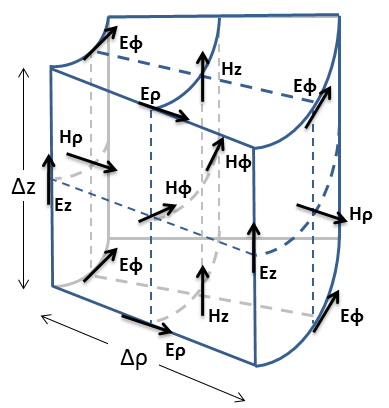
\includegraphics[width=0.5\linewidth]{pics/FDTD_cill}
	\caption{Трехмерная сетка для цилиндрической СК.}
	\label{fig:fdtd_3d}
\end{figure}

Для приведения численной схемы к требуемой в данной задаче, необходимо убрать зависимость от $z$, и представить зависимость от $\varphi$ как \eqref{eq:razdel_per}. То есть сетка визуально будет выглядеть одномерно, в расчетах будет использоваться одномерная зависимость поля и токов от $r$, однако на самом деле сетка будет являться двумерной, но с заданной зависимостью от одной из переменных. Это объясняет наличие в точках с половинчатым шагом $r=r\left(N+1/2\right)$, сразу двух компонент $H_{z}$ и $E_{r}$ с учетом того, что для разделения переменных и написании разностной схемы необходимо <<разнести>> в пространстве все исследуемые компоненты. Стоит отметить, что по причине разделения компонент в пространстве необходимо аналогичным образом разделить и временную сетку, то есть расчет фактически ведётся по половине шага, с чередованием рассчитываемых полей, аналогично расчетам по пространству.
\begin{figure}[H]\centering
	\begin{tikzpicture}
	\draw[ultra thin,->] (0,0.5)--(11,0.5);\node[below] at (11,0.5){\huge $r$};\node[left]at(0,0.5) {\large$0$};  
	\draw[thick,->] (0,0)--(0,1);\node[pin={[thick]90:{\large{$E_{\varphi},H_{r},E_{z}|_{0}$}}}]at (0,1){};
	\draw[thick,->] (2,0)--(2,1);\node[above right]at(2,0){\large{$dr$}};
	\draw[thick,->] (4,0)--(4,1);\draw[->,thick](0.5,0.5)--(1.5,0.5);\node[pin={[thick]270:{\large{$E_{r},H_{\varphi}|_{\frac{dr}{2}}$}}}]at (1.5,0.5){};\node[pin={[thick]85:{\large{$H_{z}|_{\frac{dr}{2}}$}}}]at (1,0.5){};
	\draw[thick,->] (6,0)--(6,1);\draw[->,thick](2.5,0.5)--(3.5,0.5);
	\draw[thick,->] (8,0)--(8,1);\draw[->,thick](4.5,0.5)--(5.5,0.5);
	\draw[->,thick](6.5,0.5)--(7.5,0.5);
	\draw[->,thick](8.5,0.5)--(9.5,0.5);
	\draw(1,0.5)circle[radius=0.25];\draw[fill=black](1,0.5)circle[radius=0.1];
	\draw(3,0.5)circle[radius=0.25];\draw[fill=black](3,0.5)circle[radius=0.1];
	\draw(5,0.5)circle[radius=0.25];\draw[fill=black](5,0.5)circle[radius=0.1];
	\draw(7,0.5)circle[radius=0.25];\draw[fill=black](7,0.5)circle[radius=0.1];
	\draw(9,0.5)circle[radius=0.25];\draw[fill=black](9,0.5)circle[radius=0.1];	
\end{tikzpicture}
	\label{fig^fdtd_1d}
\end{figure}

\subsection{Параметры системы. Обезразмеривание}

Решения одинаковых точных уравнений, аналогичных тем, что рассматриваются в данной работе, могут кардинально различаться в зависимости от заданных в постановке задачи параметров. Причем речь идёт не об ошибках в решении, возникающих при несоблюдении различных условий устойчивости. Под разницей в  решениях понимается разница корректных, точных аналитических решений, аналогично достижимых численными методами. Изменяется энергетические, частотные, мощностные и другие характеристики системы.

Основные уравнения представляют собой компоненты $E, H, J$ как размерные величины, т.е. полученные точные решения будут являться значениями полей и токов в системе СГС ввиду того, что сами точные уравнения изначально написаны в этой системе. Для упрощения анализа полученных данных данные уравнения требуется «обезразмерить», т.е. сделать такую замену $\tilde{E}$, $\tilde{H}$, $\tilde{\nu}$, $\tilde{r}$ и $\tilde{t}$, чтобы эти величины являлись безразмерными, но при этом также связанными между собой.

Последовательно обезразмериваем:
\begin{itemize}
	\item Плотность тока $\vec{\widetilde{j}}=\vec{j}/j_{0}$;	
	\item Напряженность магнитного и электрического полей соответственно\\ $\vec{\widetilde{H}}=\vec{H}\left(\omega_{p0}/4\pi j_{0}\right)$ и $\vec{\widetilde{E}}=\vec{E}\left(\omega_{p0}/4\pi j_{0}\right)$;	
	\item Радиальную координату $\widetilde{r}=r\omega_{p0}/c$ (все параметры, связанные с радиусом цилиндра обезразмерены аналогично);	
	\item Частоту соударений электронов с тяжелыми частицами $\widetilde{\nu}=\nu/\omega_{p0}$;	
	\item Время $\tilde{t}=\omega_{p0} t$.	
	\item Скорость распространения ионизационного фронта $V = \tilde{V}\cdot c$
\end{itemize}

В качестве основных параметров системы задавались:  частота соударений нормированная на максимальную плазменную частоту $\tilde{\nu}=\nu/\omega_{p 0}$, внешний обезразмеренный радиус цилиндра $\tilde{R}_{2}$ и безразмерное выражение $\delta=\left(R_{2}-R_{1}\right)/\\/R_{2}$ характеризующее размер области спадания плазменной концентрации и частоты $\omega_{p 0}$ относительно размеров самого цилиндра (рис. \ref{ris:f(r)} и рис. \ref{pic:cill}).

Используя описанную выше схему решения задачи, а также сетку на рис. \ref{fig:fdtd_3d}, получаем окончательную систему уравнений:

\begin{equation}
	\begin{cases}
		E_{r}|^{i+\frac{1}{2}}_{n+1}=E_{r}|^{i+\frac{1}{2}}_{n}+\frac{c\triangle\xi}{\sin^{2}\theta} \left(\frac{1}{r}H_{z}|^{i+\frac{1}{2}}_{n-\frac{1}{2}}+\frac{\cos\theta}{\Delta r}\left(E_{z}|_{n}^{i+1}-E_{z}|_{n}^{i-\frac{1}{2}}\right)-\frac{4\pi}{с} j_{r}|^{i}_{n}\right)\\
		E_{\varphi}|^{i-\frac{1}{2}}_{n+\frac{1}{2}}=E_{\varphi}|^{i-\frac{1}{2}}_{n-\frac{1}{2}}+\frac{c\Delta\xi}{\sin^{2}\theta}\left(-\cos\theta\frac{1}{r}E_{z}|_{n-\frac{1}{2}}^{i-\frac{1}{2}}-\frac{H_{z}|^{i}_{n-\frac{1}{2}}-H_{z}|^{i-1}_{n-\frac{1}{2}}}{\Delta r}-\frac{4\pi}{c} j_{\varphi}|^{i-\frac{1}{2}}_{n-\frac{1}{2}}\right)\\
		E_{z}|^{i-\frac{1}{2}}_{n+1}=E_{z}|^{i-\frac{1}{2}}_{n}+\frac{c\Delta\xi}{r}\left(\frac{\left(rH_{\varphi}\right)|^{i}_{n}-\left(rH_{\varphi}\right)|^{i-1}_{n}}{\Delta r}-H_{r}|^{i-\frac{1}{2}}_{n+\frac{1}{2}}\right)-4\pi\Delta\xi j_{z}|^{i-\frac{1}{2}}_{n}\\			H_{r}|^{i-\frac{1}{2}}_{n+\frac{1}{2}}=H_{r}|^{i-\frac{1}{2}}_{n-\frac{1}{2}}+\frac{c\Delta\xi}{\sin^{2}\theta}\left(\frac{1}{r}E_{z}|^{i-\frac{1}{2}}_{n}+\cos\theta\left(\frac{H_{z}|^{i}_{n}-H_{z}|^{i-1}_{n}}{\Delta r}+\frac{4\pi}{c}j_{\varphi}|^{i-\frac{1}{2}}_{n}\right)\right)\\
		H_{\varphi}|^{i}_{n+1}=H_{\varphi}|^{i}_{n}+\frac{c\Delta\xi}{\sin^{2}\theta}\left(\cos\theta\left(\frac{1}{r}H_{z}|^{i}-\frac{4\pi}{c}j_{r}|^{i}\right)+\frac{E_{z}|^{i+\frac{1}{2}}-E_{z}|^{i-\frac{1}{2}}}{\Delta r}\right)\\
		H_{z}|^{i}_{n+\frac{1}{2}}=H_{z}|^{i}_{n-\frac{1}{2}}+\frac{c\Delta\xi}{r}\left(-E_{r}|^{i}_{n}-\frac{(rE_{\varphi})|^{i+\frac{1}{2}}_{n+\frac{1}{2}}-(rE_{\varphi})|^{i-\frac{1}{2}}_{n+\frac{1}{2}}}{\Delta r}\right)\\
		j_{r}|^{i}_{n+1}=(1-\nu\triangle\xi) j_{r}|^{i}_{n}+\frac{\triangle\xi\omega_{p0}^{2}}{4\pi} f(r)E_{r}|^{i}_{n}\\
		j_{\varphi}|^{i-\frac{1}{2}}_{n+\frac{1}{2}}=(1-\nu\triangle\xi) j_{\varphi}|^{i-\frac{1}{2}}_{n-\frac{1}{2}}+\frac{\triangle\xi\omega_{p0}^{2}}{4\pi}f(r)E_{\varphi}|^{i-\frac{1}{2}}_{n-\frac{1}{2}}\\
		j_{z}|^{i-\frac{1}{2}}_{n+1}=(1-\nu\triangle\xi)j_{z}|^{i-\frac{1}{2}}_{n}+\frac{\triangle\xi\omega_{p0}^{2}}{4\pi} f(r)E_{z}|^{i-\frac{1}{2}}_{n}
	\end{cases}
\end{equation}
	
	\begin{multline*}
		\left.E_{r}\right|_{i+\frac{1}{2},j,k}=\left.E_{r}\right|_{i+\frac{1}{2},j,k}+\\+\frac{\Delta\xi}{\sin^{2}\theta}\left(\frac{\left.H_{z}\right|_{i+\frac{1}{2},j+\frac{1}{2},k}}{r}+\frac{\cos\theta}{\Delta r}\left(\left.E_{z}\right|_{i+1,j,k+\frac{1}{2}}-\left.E_{z}\right|_{i,j,k+\frac{1}{2}}\right)-\frac{4\pi}{c}\left.j_{r}\right|_{i+\frac{1}{2},j,k}\right)
	\end{multline*}
	\begin{multline*}
		\left.E_{\varphi}\right|_{i,j+\frac{1}{2},k}=\left.E_{\varphi}\right|_{i,j+\frac{1}{2},k}+\\
		+\frac{\Delta\xi}{\sin^{2}\theta}\left[-\frac{\cos\theta}{r}\left.E_{z}\right|_{i,j,k+\frac{1}{2}}-\frac{1}{\Delta r}\left(\left.H_{z}\right|_{i+\frac{1}{2},j+\frac{1}{2},k}-\left.H_{z}\right|_{i-\frac{1}{2},j+\frac{1}{2},k}\right)-\right.\\
		\left.-\frac{4\pi}{c}\left.j_{\varphi}\right|_{i,j+\frac{1}{2},k} \right]		
	\end{multline*}
	\begin{multline*}
		\left.E_{z}\right|_{i,j,k+\frac{1}{2}}=\left.E_{z}\right|_{i,j,k+\frac{1}{2}}+\\+\frac{c\Delta\xi}{r}\left(\frac{\left.rH_{\varphi}\right|_{i+\frac{1}{2},j,k+\frac{1}{2}}-\left.rH_{\varphi}\right|_{i-\frac{1}{2},j,k+\frac{1}{2}}}{\Delta r}-\left.H_{r}\right|_{i,j+\frac{1}{2},k+\frac{1}{2}}\right)-\left.4\pi\Delta\xi j_{z}\right|_{i,j,k+\frac{1}{2}}
	\end{multline*}
	\begin{multline*}
		\left.H_{r}\right|_{i,j+\frac{1}{2},k+\frac{1}{2}}=\left.H_{r}\right|_{i,j+\frac{1}{2},k+\frac{1}{2}}+\\
		+\frac{\Delta\xi}{\sin^{2}\theta}\left[\frac{\left.E_{z}\right|_{i,j,k+\frac{1}{2}}}{r}+\cos\theta\left(\frac{\left.H_{z}\right|_{i+\frac{1}{2},j+\frac{1}{2},k}-\left.H_{z}\right|_{i-\frac{1}{2},j+\frac{1}{2},k}}{\Delta r}+\frac{4\pi}{c}\left.j_{r}\right|_{i,j+\frac{1}{2},k}\right)\right]
	\end{multline*}
	\begin{multline*}
		\left.H_{\varphi}\right|_{i+\frac{1}{2},j,k+\frac{1}{2}}=\left.H_{\varphi}\right|_{i+\frac{1}{2},j,k+\frac{1}{2}}+\\
		+\frac{\Delta\xi}{\sin^{2}\theta}\left[\cos\theta\left(\frac{\left.H_{z}\right|_{i+\frac{1}{2},j+\frac{1}{2},k}}{r}-\frac{4\pi}{c}\left.j_{r}\right|_{i+\frac{1}{2},j,k}\right)+\frac{\left.E_{z}\right|_{i+1,j,k+\frac{1}{2}}-\left.E_{z}\right|_{i,j,k+\frac{1}{2}}}{\Delta r}\right]
	\end{multline*}
	\begin{multline*}
		\left.H_{z}\right|_{i+\frac{1}{2},j+\frac{1}{2},k}=\left.H_{z}\right|_{i+\frac{1}{2},j+\frac{1}{2},k}-\\
		-\frac{c\Delta\xi}{r}\left(\frac{\left.rE_{\varphi}\right|_{i+1,j+\frac{1}{2},k}-\left.rE_{\varphi}\right|_{i,j+\frac{1}{2},k}}{\Delta r}+\left.E_{r}\right|_{i+\frac{1}{2},j,k}\right)
	\end{multline*}
	\begin{equation*}
		\begin{cases*}
			j_{r}|_{i+\frac{1}{2},j,k}=(1-\nu\triangle t) j_{r}|_{i+\frac{1}{2},j,k}+\frac{\triangle t\omega_{p0}^{2}}{4\pi} f(r)E_r|_{i+\frac{1}{2},j,k}\\
			j_{\varphi}|_{i,j+\frac{1}{2},k}=(1-\nu\triangle t) j_{\varphi}|_{i,j+\frac{1}{2},k}+\frac{\triangle t\omega_{p0}^{2}}{4\pi}f(r)E_{\varphi}|_{i,j+\frac{1}{2},k}\\
			j_{z}|_{i,j,k+\frac{1}{2}}=(1-\nu\triangle t) j_{z}|_{i,j,k+\frac{1}{2}}+\frac{\triangle t\omega_{p0}^{2}}{4\pi}f(r)E_{z}|_{i,j,k+\frac{1}{2}}
		\end{cases*}
	\end{equation*}
	\begin{equation*}
		\begin{cases*}
			\left.H_{\varphi}\right|_{i+\frac{1}{2}}=\left.H_{\varphi}\right|_{i+\frac{1}{2}}+\frac{\Delta\xi}{\sin^{2}\theta}\left[\cos\theta\left(\frac{\left.H_{z}\right|_{i+\frac{1}{2}}}{r}-\frac{4\pi}{c}\left.j_{r}\right|_{i+\frac{1}{2}}\right)+\frac{\left.E_{z}\right|_{i+1}-\left.E_{z}\right|_{i}}{\Delta r}\right]\\
			\left.H_{z}\right|_{i+\frac{1}{2}}=\left.H_{z}\right|_{i+\frac{1}{2}}-\frac{c\Delta\xi}{r}\left(\frac{\left.rE_{\varphi}\right|_{i+1}-\left.rE_{\varphi}\right|_{i}}{\Delta r}+\left.E_{r}\right|_{i+\frac{1}{2}}\right)\\
			j_{r}|_{i+\frac{1}{2}}=(1-\nu\triangle t) j_{r}|_{i+\frac{1}{2}}+\frac{\triangle t\omega_{p0}^{2}}{4\pi} f(r)E_r|_{i+\frac{1}{2},j,k}\\
			j_{\varphi}|_{i}=(1-\nu\triangle t) j_{\varphi}|_{i}+\frac{\triangle t\omega_{p0}^{2}}{4\pi}f(r)E_{\varphi}|_{i}\\
			j_{z}|_{i}=(1-\nu\triangle t) j_{z}|_{i}+\frac{\triangle t\omega_{p0}^{2}}{4\pi}f(r)E_{z}|_{i}
		\end{cases*}
	\end{equation*}
%	\begin{equation*}
%		
%	\end{equation*}
%	\begin{equation*}
%		
%	\end{equation*}
%	\begin{equation*}
%		
%	\end{equation*}

где по $n$ откладываются шаги по времени, а по $i$ -- шаги по $r$.
\newpage
\subsection{Условия поглощения}

Для предотвращения <<загрязнения>> сигнала отражениями с другого конца оси $r$, то есть аналитически при $r\rightarrow\infty$ недостаточно только обнулить производную саму функцию на конце границы расчета. В зависимости от поставленной задачи и моделируемой области могут использоваться различные граничные условия. Чаще всего используются условие идеально согласованных слоев \textit{(perfectly matched layers -- PML)}, периодические условия для расчета периодических структур и условия идеального проводника на границе, когда в граничных
точках поле берется всегда равным нулю. Последнее имеет очень серьезный недостаток, так как от такой границы идет полное отражение волны, и если требуется длительное
наблюдение электромагнитного поля, отраженные от границ счетной области волны могут <<загрязнять>> сигнал и делать невозможным его дальнейший анализ. Для исключения отражения от границ области и был придуман способ идеально-согласованных слоев, описанный в \cite{fdtd_pml}. В данной работе используются только условие идеально согласованных слоев, когда в определенной области расчетной сетки вводятся слои, поглощающие попадающее в него поле (расчет поглощения для токов существенно усложнил бы задачу, поэтому поглощение происходит в расчетном вакууме), причем относительно каждого отдельного слоя среда и её свойства изменяются несущественно, однако усиление поглощающих свойств происходит при продвижение от начала данных слоёв до их конца (обычно это происходит на границе расчетной области), где поглощение усиливается до максимума и дальнейшего прохода энергии через последний слой невозможно.

В частности, для PML, предназначенного для поглощения волн, распространяющихся в направлении r, как в данной работе, в волновое уравнение включено следующее преобразование. Всякая производная  $\partial/\partial r$ заменяется на:

\begin{equation}
	\frac{\partial}{\partial r} \to \frac{1}{1 + \frac{i\sigma(r)}{\omega}} \frac{\partial}{\partial r}
\end{equation}
где $ \omega$ -- угловая частота поглощаемой волны и $\sigma$ - некоторая функция от $r$, отвечающая за поглощение слоя в точке $r$.  То есть $dr \to dr (1 + i\sigma(r)/\omega)$.

\subsection{Условие устойчивости разностной схемы}

При составлении пространственно-временных реализаций пространство и время, соответственно, поддаются дискретизации, и уже если и воспроизводят реальную картину исследуемого объекта, поля и.т.д., то с определенной неточностью. Можно также упомянуть тот факт, что все расчеты в численных методах производятся с помощью вычислительных машин (компьютеров), то есть к неточности дискретизации также добавляется машинная неточность самого компьютера.

В случае, рассматриваемом в данной работе, условием устойчивости метода конечных разностей является так называемое условие (критерий) Куранта -- Фридрихса -- Леви, или просто условие Куранта \cite{courant1945}.

В текущей задаче и в цилиндрической СК это условие \eqref{eq:courant} будет выглядеть так:
\begin{equation}
	\Delta\xi\leq\frac{\Delta r}{c\sqrt{2}}
	\label{eq:courant}
\end{equation}

В свою очередь условие устойчивости для $\Delta r$ будет следующим:
\begin{equation}
	\Delta r\ll\dfrac{\nu}{\omega_{p 0}}\left(R_{2}-R_{1}\right)
	\label{eq:courant_1}
\end{equation}








\newpage
\section{Эффективность энергетических преобразований}

Основной задачей, поставленной в данной работе, является определение оптимальных параметров (размеров) системы, при которых достигается максимально эффективное преобразование энергии, запасенной в образованном в момент мгновенной ионизации остаточном токе, в электромагнитную энергию излучения. Дальнейшие исследования полученных решений можно свести к изучению излучения волны, возбуждаемой данной системой (данным цилиндром) в вакуум. С учетом того, что цилиндр, представленный в данной задаче, является бесконечным, с бесконечно быстро распространяющимся фронтом ионизации, расчёт коэффициента полезного действия по определению сводится к нахождению отношения суммарной энергии, излученной системой за всё время к суммарной энергии, запасенной в цилиндре во всем пространстве. При этом обе энергии в виду бесконечности цилиндра, будут рассчитываться на единицу его длины. 


\subsection{Энергия, запасенная в остаточном токе}
Для дальнейших выводов воспользуемся соотношением:
\begin{equation}
	W_{k}=\frac{mv^2}{2} 
	\label{3}
\end{equation}

а также воспользуемся соотношениями \eqref{j:eNv} и \eqref{eq:omega_p0}.
Уравнение \eqref{eq:omega_p0} есть определение зависимости плазменной частоты $\omega_{p}$ от $N(r)$.	Уравнение \eqref{j:eNv} -- определение плотности тока в проводнике как упорядоченного движения электронов в нём. Уравнение \eqref{3} --  кинетической энергии электрона, где $m$ $-$  его	масса, $v$ -- его скорость.

Для нахождения запасенной энергии в токе (или же кинетической энергии электронов на единицу длины, а не на единицу объёма)
\begin{equation}
	W_{\text{запасенная}}=W_{\text{кин ед дл}}=\iint W_{\text{кин ед об}}dS
	\label{W_kl}
\end{equation}
$-$ интеграл по поперечному сечению цилиндра $dS$ от $r=0$ до $r = R_2$. \newpage Кинетическая энергия системы является функцией от $r$ и находится как произведение плазменной концентрации $N(r)$ и кинетической энергии одного электрона \eqref{3}.
\begin{equation}
	W_{\text{кин ед об}}=N\left(r\right)\frac{mv^2}{2}
	\label{W_kV}
\end{equation}


Таким образом выражение для энергии запасенной в системе на единицу длины цилиндра приобретает следующий вид: 

\begin{equation}
	W_{\text{запасенная}}=W_{\text{зап}}=\iint N(r)\frac{mv^2}{2}dS=\frac{m}{2}\iint Nv^{2}dS
\end{equation}

Из	\eqref{j:eNv} мы можем получить $Nv=j/e$, а также $v=j/Ne$. Получим: 

\begin{equation}
	W_{\text{зап}}=\frac{m}{2}\iint\frac{j}{e}\cdot\frac{j}{eN} dS=\frac{m}{2e^2}\iint\frac{j^2}{N} dS
\end{equation}
\quad Из (\ref{3}) мы можем получить выражение для $N(r)$.

\begin{equation}
	N(r)=\frac{\omega_{p}^{2}(r)m_{e}}{4\pi e^{2}}=\left[\omega_{p}^{2}=\omega_{p 0}^{2}\cdot f(r)\right]=\frac{\omega_{p 0}^{2}m_{e}}{4\pi e^{2}}\cdot f(r)
\end{equation}
Учитывая, что энергия <<запасается>> в начальный момент времени, значит и выражение для плотности тока мы должны искать по начальному распределению, то есть по начальному условию:
\begin{equation}
	j(r)|_{t=0}=j_{0}f(r)
\end{equation}
\begin{equation}
	W_{\text{зап}}=\frac{m}{2e^2}\iint\frac{j^2}{N} dS=\frac{m_{e}}{2e^{2}}\cdot \frac{4\pi e^{2}}{\omega_{p 0}^{2}m_{e}}\cdot j_{0}^{2}\iint\frac{f(r)^{2}}{f(r)}dS
\end{equation}


После сокращений и преобразований получаем:					
\begin{equation}
	W_{\text{зап}}=2\pi\left(\frac{j_{0}}{\omega_{p 0}}\right)^{2}\iint f(r)dS
\end{equation}
В интеграле по области $S$ в цилиндрической системе координат элемент $dS=rdrd\varphi$ 
\begin{equation}
	W_{\text{зап}}=2\pi\left(\frac{j_{0}}{\omega_{p 0}}\right)^{2}\int_{0}^{2\pi}d\varphi\int_{0}^{R_{2}} rf(r)dr=\newline
	=\left(\frac{2\pi j_{0}}{\omega_{p 0}}\right)^{2}\int_{0}^{R_{2}} rf(r)dr
\end{equation}

\begin{eqnarray}
	\int_{0}^{R_{2}}rf(r)dr=\int_{0}^{R_{1}}rdr+\int_{R_{1}}^{R_{2}}rf(r)dr \\
	\int_{0}^{R_{2}}rf(r)dr=\frac{R_{1}^{2}}{2}+\int_{R_{1}}^{R_{2}}rf(r)dr=\frac{R_{1}^{2}}{2}+{\bf I}
\end{eqnarray}

Где ${\bf I}=\int\limits_{R_{1}}^{R_{2}}r cos^{2}\left(\frac{\pi(r-R_{1})}{2(R_{2}-R_{1})}\right)dr=\left(R_{2}^{2}-R_{1}^{2}\right)/4$

\begin{multline}
	W_{\text{зап}}=\left(\frac{2\pi j_{0}}{\omega_{p 0}}\right)^{2}\int_{0}^{R_{2}} rf(r)dr=\\
	=\left(\frac{2\pi j_{0}}{\omega_{p 0}}\right)^{2} \left(\frac{R_{1}^{2}}{2}+\frac{R_{2}^{2}-R_{1}^{2}}{4}\right)=\\
	=\left(\frac{2\pi j_{0}}{\omega_{p 0}}\right)^{2}\left(\frac{R_{1}^{2}+R_{2}^{2}}{4}\right)
\end{multline}
\quad Получаем окончательное уравнение (\ref{W_zap}) для запасенной энергии:
\begin{equation}
	W_{\text{зап}}=\left(\frac{\pi j_{0}}{\omega_{p 0}}\right)^{2}\left(R_{1}^{2}+R_{2}^{2}\right)
	\label{W_zap}
\end{equation}

\newpage
\subsection{Энергия излученная системой.\\ Коэффициент полезного действия}

Энергия, преобразованная в излученную, по определению есть циркуляция продольной компоненты (в нашем случае, это компонента, направленная вдоль вектора распространения волны, то есть координате $r$) вектора Пойнтинга по замкнутому контуру, охватывающего сечение цилиндра.

Для получения конечного выражения для излученной энергии это выражение мы должны проинтегрировать по всему времени от $0$ до $\infty$, чтобы получить значение излученной энергии на всем промежутке времени, то есть:

\begin{multline}
	W_{\text{излученная на единицу длины}}=W_{\text{изл}}=\int\limits_{0}^{\infty}\left[\oint S_{r}dl\right]dt=\\
	=\int\limits_{0}^{\infty}\left[\int\limits_{0}^{2\pi} S_{r}rd\varphi\right]dt=\\
	\left[
	\vec{S}=\begin{vmatrix}
		\vec{r}_{0}& \vec{\varphi}_{0}& \vec{z}_{0}\\
		E_{r}& E_{\varphi}& E_{z}\\
		H_{r}& H_{\varphi}& H_{z}\\
	\end{vmatrix};\quad S_{r}=\left(E_{\varphi}H_{z}-E_{z}H_{\varphi}\right)\right]\\
	=\frac{c}{4\pi}\int\limits_{0}^{\infty}\left[\int\limits_{0}^{2\pi}\left(E_{\varphi}H_{z}-E_{z}H_{\varphi}\right)rd\varphi\right]dt
	\label{eq:W_izl}
\end{multline}

Используя ранее сзаданную зависимость компонент $E$ и $H$ от угла $\varphi$ \eqref{eq:razdel_per}, избавимся от соответствующего интеграла и получим окончательное выражение для $W_{\text{изл}}$:
\begin{equation}
	W_{\text{изл}}=\frac{cr}{4\pi}\int\limits_{0}^{\infty}\pi\left[E_{\varphi}H_{z}-E_{z}H_{\varphi}\right]dt=\frac{cr}{4}\int\limits_{0}^{\infty}(E_{\varphi}H_{z}-E_{z}H_{\varphi})dt	
\end{equation}

Запишем общее выражение для КПД в таком виде:
\begin{equation}
	\eta =\frac{W_{\text{излученная на единицу длины}}}{W_{\text{запасенная на единицу длины}}}=\frac{W_\text{изл}}{W_\text{зап}}
	\label{eq:kpd3}
\end{equation}

Коэффициент полезного действия считается используя \eqref{eq:W_izl} и \eqref{W_zap}:
\begin{equation}
	\eta=\dfrac{\dfrac{cR_{0}}{4}\int\limits_{0}^{\infty}(E_{\varphi}H_{z}-E_{z}H_{\varphi})dt}{\left(\dfrac{\pi j_{0}}{\omega_{p 0}}\right)^{2}\left(R_{1}^{2}+R_{2}^{2}\right)}
	\label{eq:kpd_last}
\end{equation}
 где интеграл в числителе легко находится с помощью численных методов нахождения интегралов заданной функции. Остальные параметры являются константными параметрами задачи.
\newpage





\newpage
\section{Результаты расчетов}

Согласно введению,  требуется  разработать вычислительный код для решения всех, полученных выше, выражений. Ввиду нецелесообразности демонстрации кода в данной работе, само <<тело>> программы мы опустим и будем работать уже с конечными результатами действия этого кода.

В ходе расчетов были выявлены и получены пространственно-временные распределения электрического и магнитного полей, токов, а также спектральные характеристики излучаемой волны для каждого отдельного набора параметров. Пример получаемой кодом картины представлен на рисунке \ref{ris:matlab}.

\begin{figure}[H]\centering	
	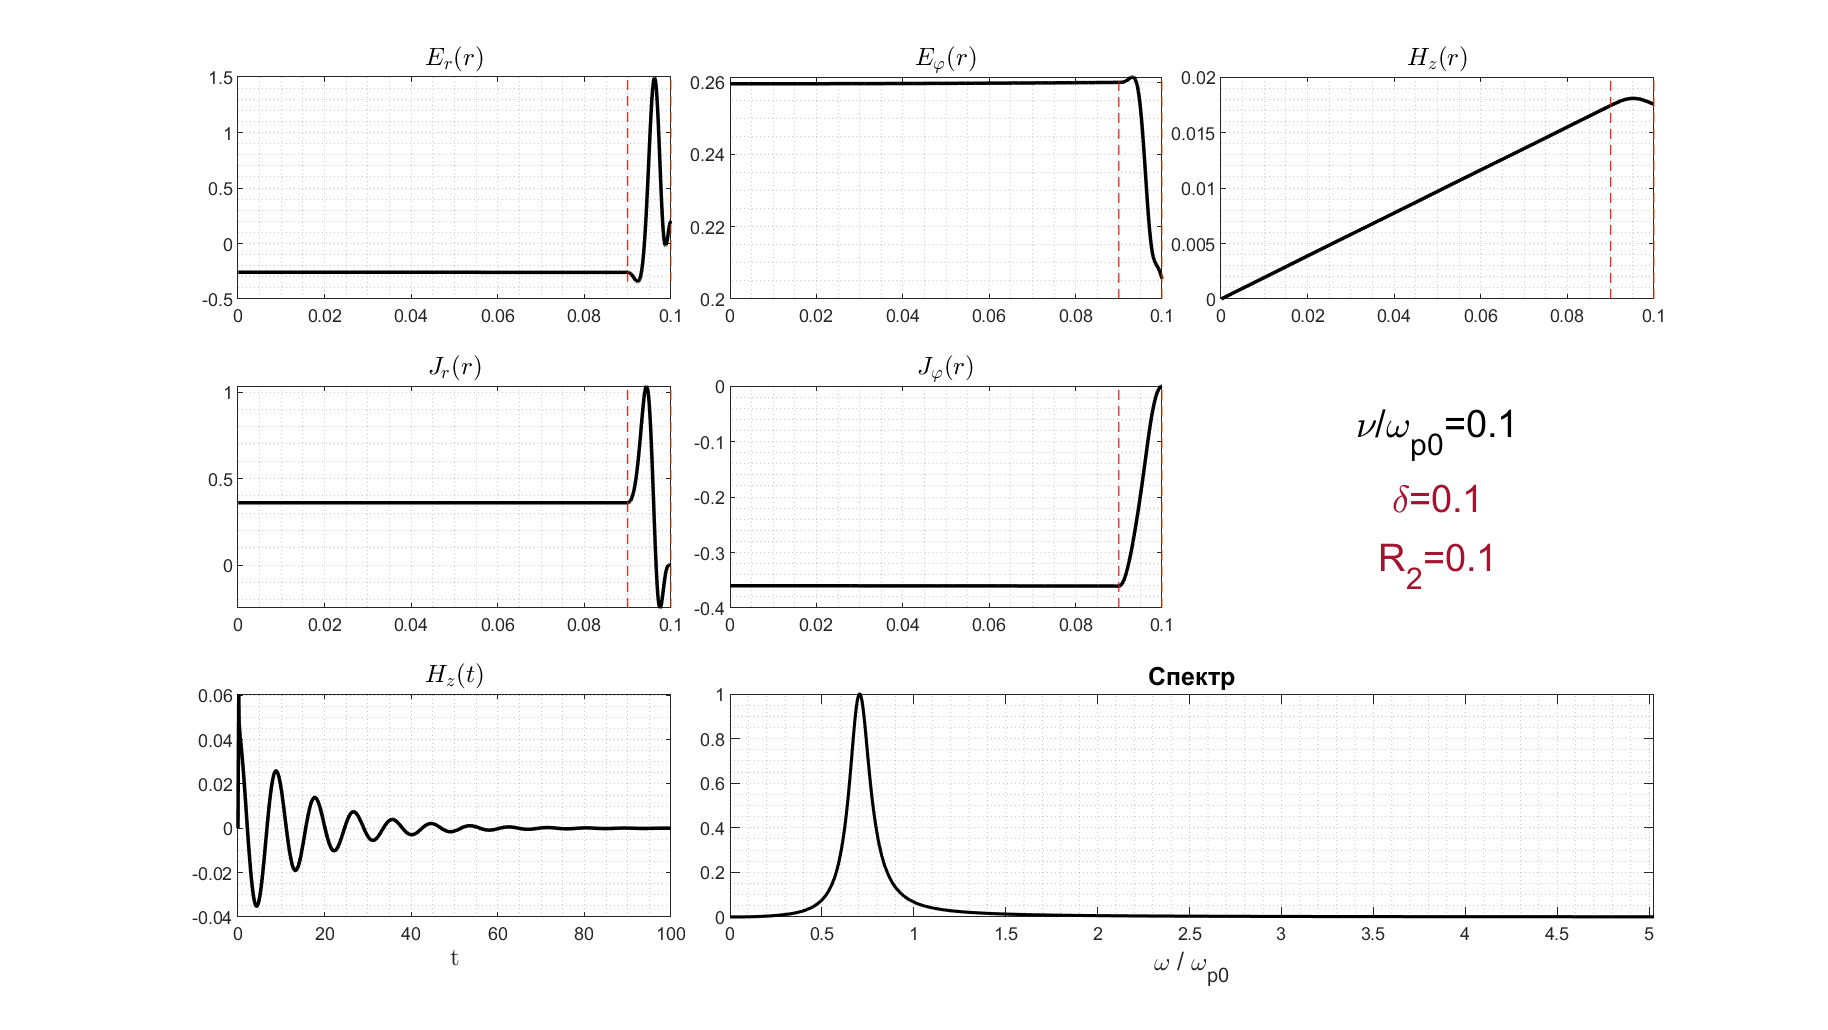
\includegraphics[width=0.9\linewidth]{pics/picture_123}
	\caption{Пространственно временная эволюция системы, а также спектр излученной волны \\ при $\nu/\omega_{p0}=0.1$, $\delta=0.1$, $R_{2}=0.1$}
	\label{ris:matlab}
\end{figure}

На нём видно, что описанная нами система излучает волну определенной формы во внешнюю среду. При рассмотрении задач с другим набором параметров системы получается волна аналогичного вида, однако разница начинает проявляться при дальнейшей обработке полученных данных.

Рассмотрим рис. \ref{ris:matlab} более детально. Обратим внимание на распределение компонент полей и токов от координаты $\left(E_{r}(r),E_{\varphi}(r),H_{z}(r),J_{r}(r),J_{\varphi}(r)\right)$. В зоне $0.09\leq r\leq 0.1$ или же $R_{1}\leq r\leq R_{2}$ отмечается резкое усиление полей и токов вокруг точки $r=\left(R_{1}+R_{2}\right)/2$. Подобный эффект называется \textit{плазменным резонансом}. В точке $r=\left(R_{1}+R_{2}\right)/2$ согласно \eqref{eq:omega_p(r)} и \eqref{eq:f(r)} локальная плазменная частота равна резонансной частоте, которую можно увидеть на спектре излучения, изображенном на рис. \ref{ris:matlab}. При подобных параметрах системы резонансная частота равна $\omega_{\text{рез}}=\omega_{p0}/\sqrt{2}$ и называется частотой \textit{геометрического резонанса}.

При расширении зоны неоднородности плазмы (при увеличении $\delta$) зона геометрического резонанса всё также остается в её середине, спектр расширяется, а сам резонанс более широко распределяется по области неоднородности.
\begin{figure}[H]\centering	
	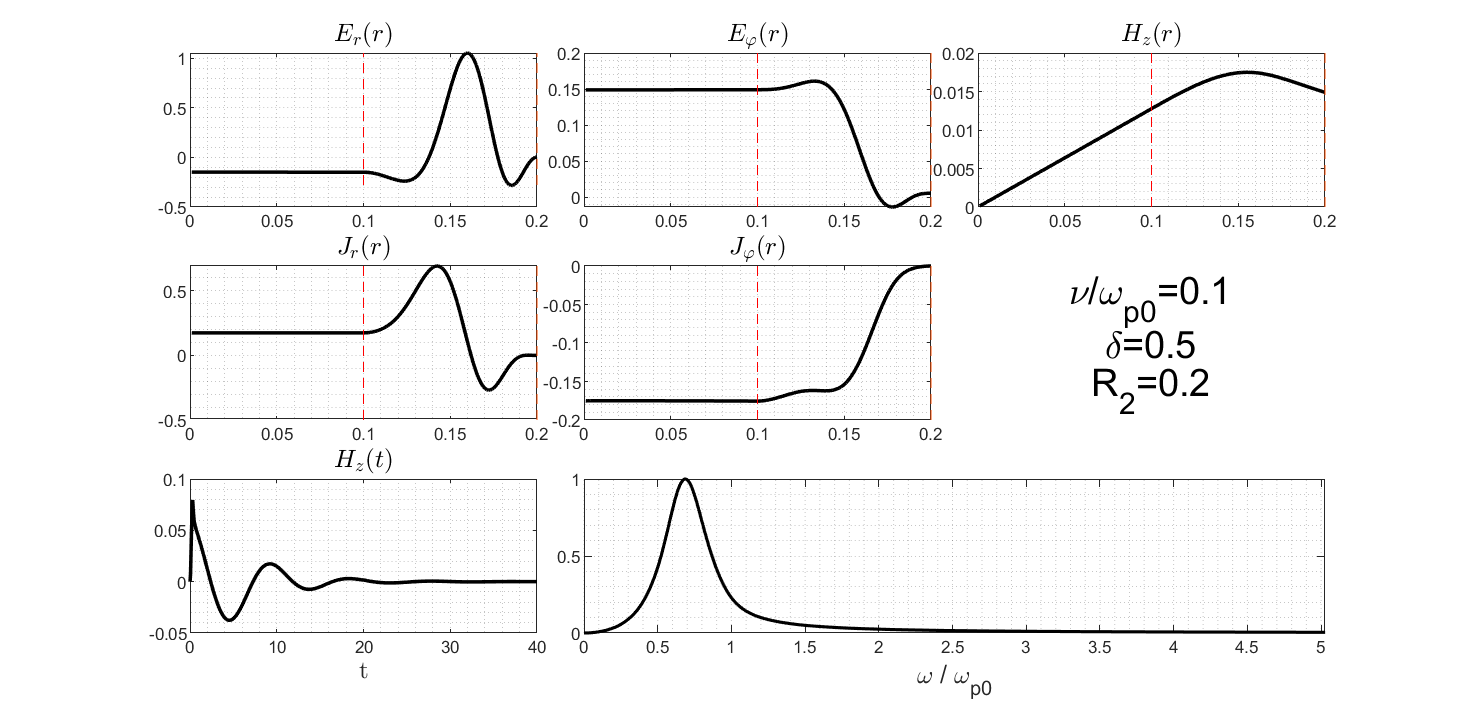
\includegraphics[width=0.9\linewidth]{pics/pic9}
	\caption{Пространственно временная эволюция системы, а также спектр излученной волны \\ при $\nu/\omega_{p0}=0.1$, $\delta=0.5$, $R_{2}=0.2$}
	\label{ris:matlab_2}
\end{figure}

Изображенные на рис. \ref{ris:matlab} и рис. \ref{ris:matlab_2} картины являются для данной работы показательными -- с одной стороны -- ввиду того, что они полностью согласуются с упомянутыми во введении исследованиями \cite{Gildenburg2007,Vved2005}, а с другой -- при численном решении данной задачи необходимо накладывать существенные условия на точность расчетов: временные и пространственные шаги должны быть критически малы, а количественно расчетов с ними должно происходить существенно больше. То есть численные ошибки и неточности вычислительной разностной схемы в случае задаче с малыми параметрами показали бы существенное отклонение и максимальное расхождение с теорией. То есть точность последующих расчетов является приемлемой, так как при численных расчетах критической задачи отклонений не обнаружено.

\subsection{Энергетические зависимости. \\Оптимальный набор параметров}

Для дальнейшего изучения системы с прикладной точки зрения имеет смысл поиск так называемого оптимума системы -- в нашем случае оптимального набора параметров и условий, при которых обеспечивается наилучшее (самое эффективное) излучение -- то есть мы должны стремиться к максимально эффективному преобразованию энергии, запасенной в остаточном токе, в энергию электромагнитного излучения заданной системы. 

Стоит также объяснить прикладной смысл и соответствующие выкладки данной работы. В реальных исследуемых моделях (конструкциях) подобный тип излучения достигается с помощью мощного короткого ионизирующего лазерного импульса, когда за несколько фемтосекунд ( $\sim10^{-15}$ сек) система из газа трансформируется в плазму (то есть происходит ионизация), при этом длительность этого импульса настолько мала, что электроны, ионы и нейтральные частицы не успевают существенно изменить свои положения в системе. То есть ионизированная система приобретает начальный импульс, который мы в уравнениях записываем как начальные условия, а уже после этого <<удара>> система начинает определенным образом эволюционировать и эту эволюцию мы и изучаем в данной работе. Ввиду таких коротких по времени возбуждениях системы, а также ввиду того, что размер системы много больше дебаевского радиуса, мы пренебрегаем температурным воздействием системы на саму себя. В данной работе это выражается в том, что уравнение для плотности тока в (\ref{eq:sys:start}) не содержит в себе прямую зависимость от температуры.

Конструкция полученной системы зависит как от типа, характера <<заряжающего>> импульса, так и от идеализации самой модели и выводов из неё, и прочих возможных допущениях, которые могут приниматься в зависимости от поставленной задачи. С изменением структуры системы, при изменении относительных размеров области спадающей границей по сравнению с участком плато наблюдается изменение колебательных свойств системы \cite{Vved2005}. Как уже говорилось выше, когда $\delta,\:\nu\rightarrow0$, то есть область неоднородности плазмы очень мала, система  имеет только одну резонансную частоту $\omega_{\text{рез}}=\omega_{p 0}/\sqrt{2}$, так называемую <<частоту геометрического резонанса>> \cite{Gilden2000}, которую можно обнаружить и с помощью данного вычислительного кода (рис. \ref{pic:spm_res}). С уменьшением частоты соударений спектр должен сужаться в пределе до дельта-функции в точке геометрического резонанса, а с увеличением, соответственно, расширяться.

\begin{figure}[H]\centering	
	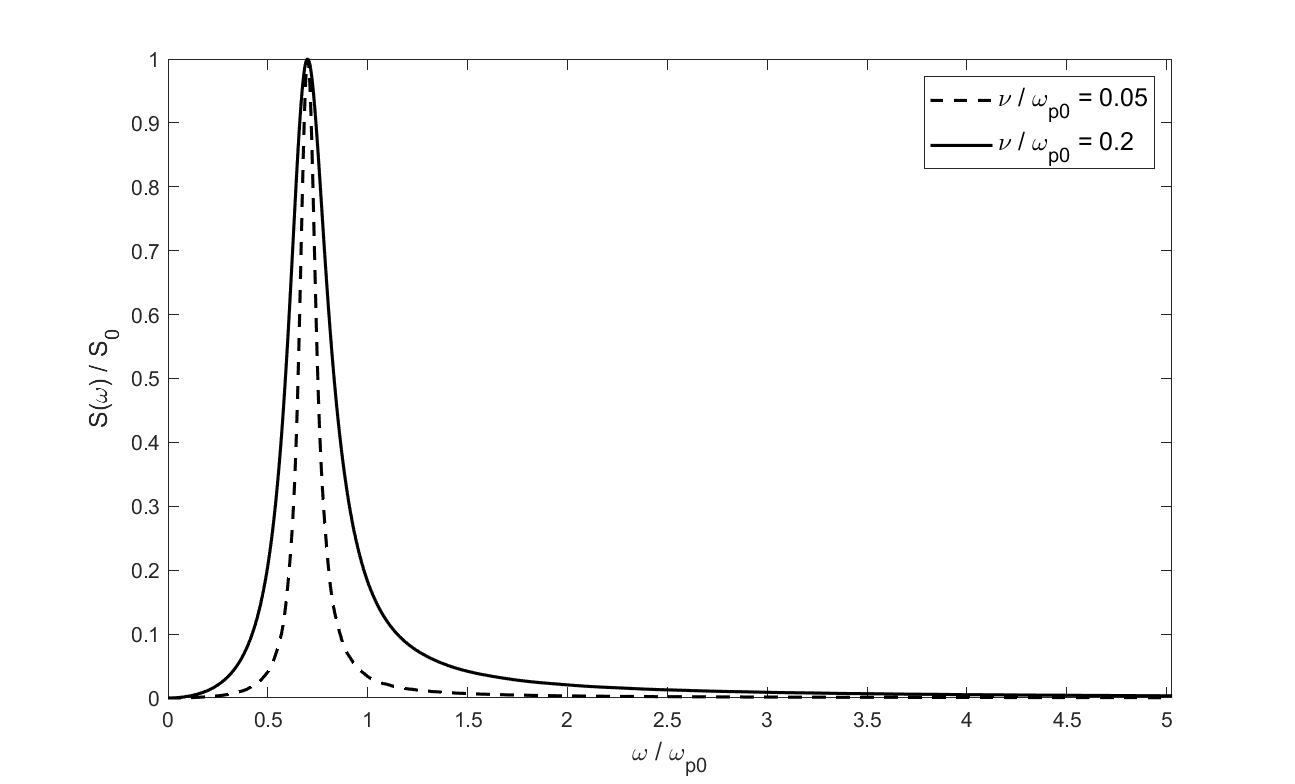
\includegraphics[scale=0.7]{pics/SPM_minimal}
	\caption{Наблюдение геометрического резонанса при $\delta=0.1, R_{2}=0.2,$  и различных значениях \\ $\nu/\omega_{p0} $ $(0.05$ и $0.2)$.}
	\label{pic:spm_res}
\end{figure}

Когда же область спадания приобретает определенный -- отличный от бесконечно малого -- размер, так как плазменная частота спадает от своего максимального значения до нуля, в этой области мы можем <<дойти>> до частоты, совпадающей с $\omega_{p 0}/\sqrt{2}$. Ввиду того, что распределение плазменной концентрации, а значит и $\omega_{p}$, не изменяется от времени, а их распределение от $r$ задано по \eqref{eq:N(r)}, $\omega_{\text{рез}}=\omega_{p 0}/\sqrt{2}$ ровно посередине области переменной концентрации (то есть, при $r=\frac{R_{1}+R_{2}}{2}$). Возникающий в данном случае эффект, когда плазменная частота совпадает с резонансной частотой, называется \textit{плазменный резонансом}. 

Возникновение плазменного резонанса порождает соответствующие энергетические потери в исследуемом объекте, причем если некоторые из возможных в данной задаче потерь всё же можно назвать полезными (например, потери радиационные -- то есть энергия теряется на излучении системы -- в их нахождении и эффективности основная суть данной работы) которые увеличивают эффективность моделируемого плазменного излучателя, а потери на соударении электронов с тяжелыми частицами можно сравнить с потерями энергии колебательных систем на затухании, то потери на резонансе --  естественно, являются потерями негативными -- однако, они напрямую зависят от ширины области неоднородной плотности плазмы, то есть от параметра $\delta$. Потери на соударении присутствуют в любой системе, где частота соударений $\nu$ ненулевая. Потери на излучении зависят от размеров системы, то есть от параметра $R_{2}$, и скорее связаны с её внутренними свойствами и способностями эффективно отдавать энергию, запасенную в остаточном токе. Подбор оптимальных параметров системы, когда энергия запасена в достаточном количестве, чтобы не поглотиться на резонансе и/или соударении, но при этом излученная энергия составляла бы б\'ольшую часть от запасенной, является основной задачей данной работы. Чем больше $\delta$, тем больше потери на резонансе преобладают над остальными потерями, что показывают расчеты на рисунке \ref{ris:kpd_r2_delta_07_1}.

Полученные расчеты поставленной задачи с множеством параметров, а также последующий расчет коэффициента полезного действия по формуле \eqref{eq:kpd_last} изображены на рисунке \ref{ris:kpd_delta_r2} (а, б).

\begin{figure}[H]	
	\begin{minipage}[H]{0.5\linewidth}
		\center{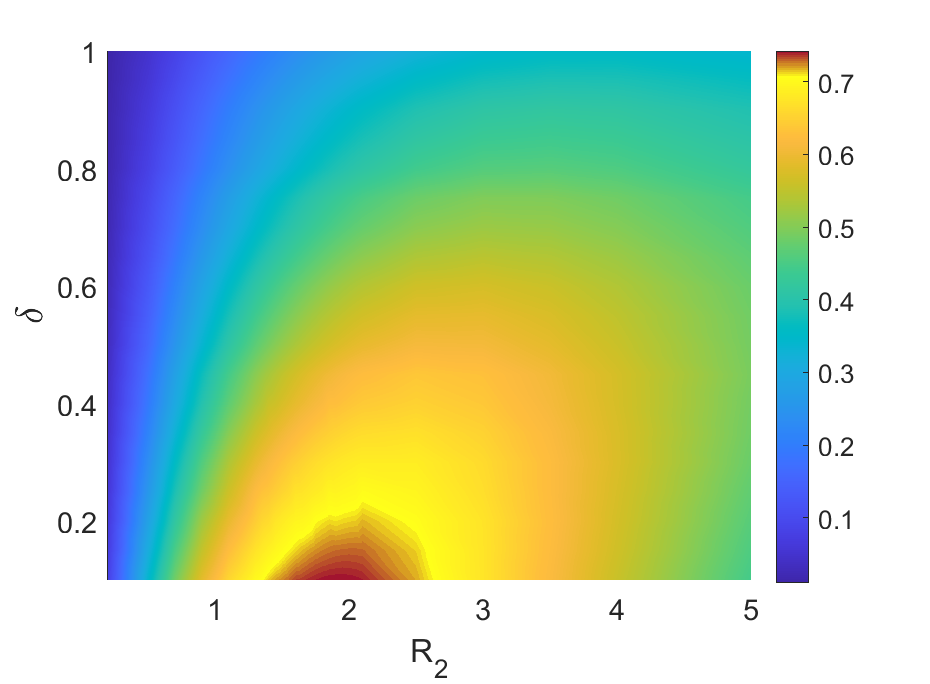
\includegraphics[width=1\linewidth]{pics/KPD_01} \\ а)}
	\end{minipage}	
	\begin{minipage}[H]{0.5\linewidth}
		\center{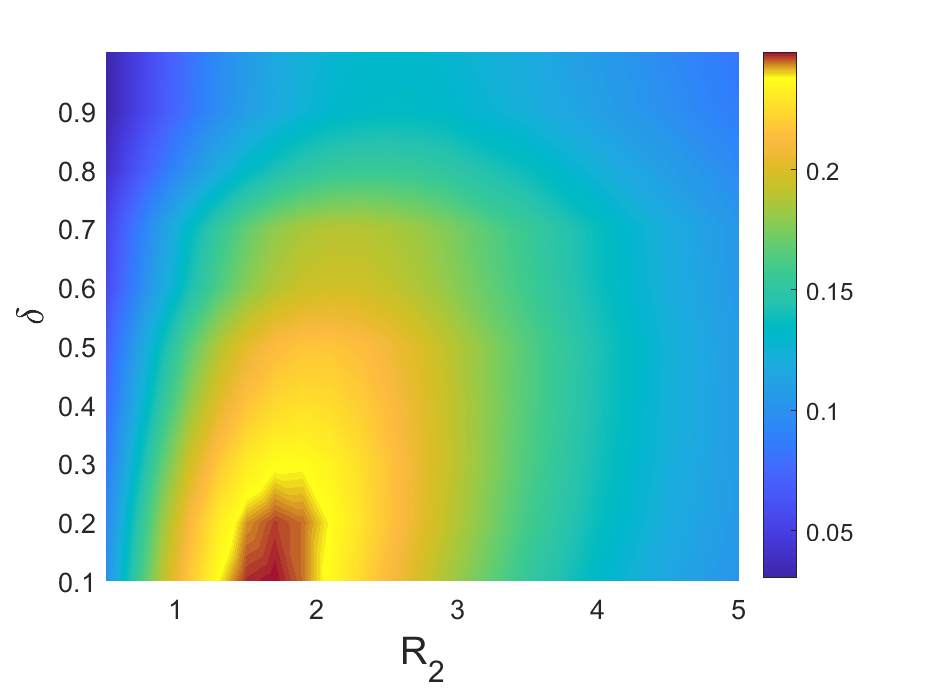
\includegraphics[width=1\linewidth]{pics/KPD_07} \\ б)}
	\end{minipage}
	\caption{Эффективность преобразования энергии, запасенной в остаточном токе в электромагнитную энергию излучения  в зависимости от радиуса цилиндра $R_{2}$ и размера неоднородной области  $\delta$ при  $\nu / \omega_{p 0}=0.1$ (а) и  $\nu / \omega_{p 0}=0.7$.}
	\label{ris:kpd_delta_r2}
\end{figure}
\newpage
Из полученных данных можно определить зону оптимальных значений $R_{2}$ и $\delta$ -- при которых КПД максимальный, то есть б\'ольшая часть энергии не переходит в негативные для нас потери, а излучается, то есть радиационные потери больше прочих. Также имеет смысл построить в оптимуме системы графики КПД от значений одного параметра при фиксированном значении другого и наоборот (рисунки \ref{ris:kpd_r2_delta_07} и \ref{ris:kpd_r2_delta_07_1}).

\begin{figure}[H]
	\centering
	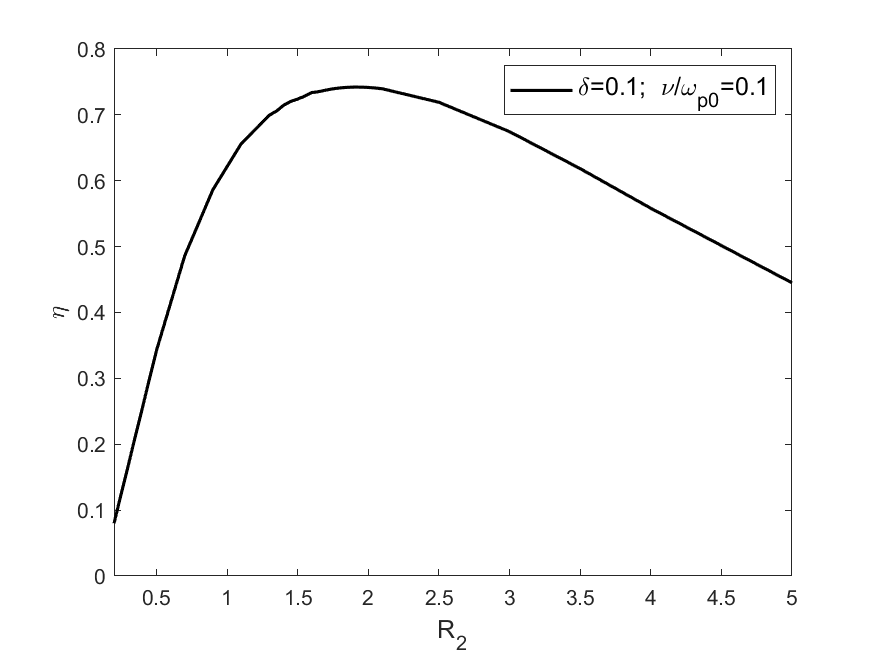
\includegraphics[scale=0.7]{pics/KPD_r2}
	\caption{Эффективность излучения при оптимальном размере неоднородной области $\delta=0.1$ в зависимости то радиуса цилиндра $R_{2}$ ($\nu / \omega_{p 0}=0.1$).}
	\label{ris:kpd_r2_delta_07}
\end{figure}

\begin{figure}[H]
	\centering
	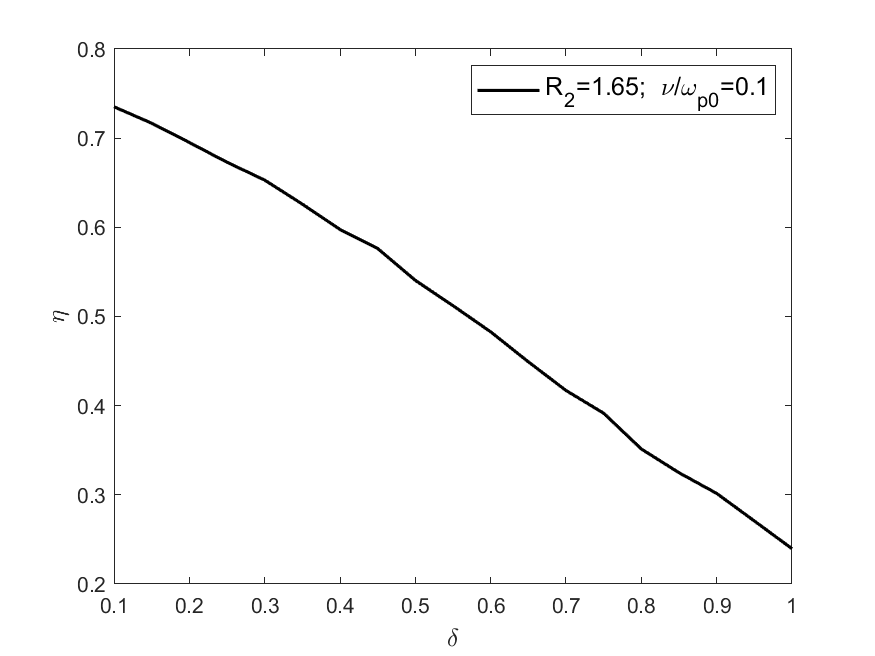
\includegraphics[scale=0.7]{pics/KPD_delta}
	\caption{Эффективность излучения при оптимальном радиусе цилиндра $R_{2}=1.64$ в зависимости от размера неоднородной области $\delta$. ($\nu / \omega_{p 0}=0.1$).}
	\label{ris:kpd_r2_delta_07_1}
\end{figure}


\newpage
Графики зависимостей КПД от нормированной частоты соударений при двух фиксированных $\delta$, что объясняет две различные ситуации, когда зона спада плазменной плотности либо мала по сравнению с общими размерами цилиндра $\left(\delta=0.1\right)$, либо составляет основную часть $\left(\delta=1\right)$, расположены на рисунке \ref{ris:kpd_nu}. Полученный рисунок объясняет, что эффективная излучаемая энергия системы падает при увеличении количества соударений в ней, то есть вместо резонансных потерь доминировать начинают уже потери на соударениях.

\begin{figure}[H]\centering
	\captionsetup{justification=centering}
	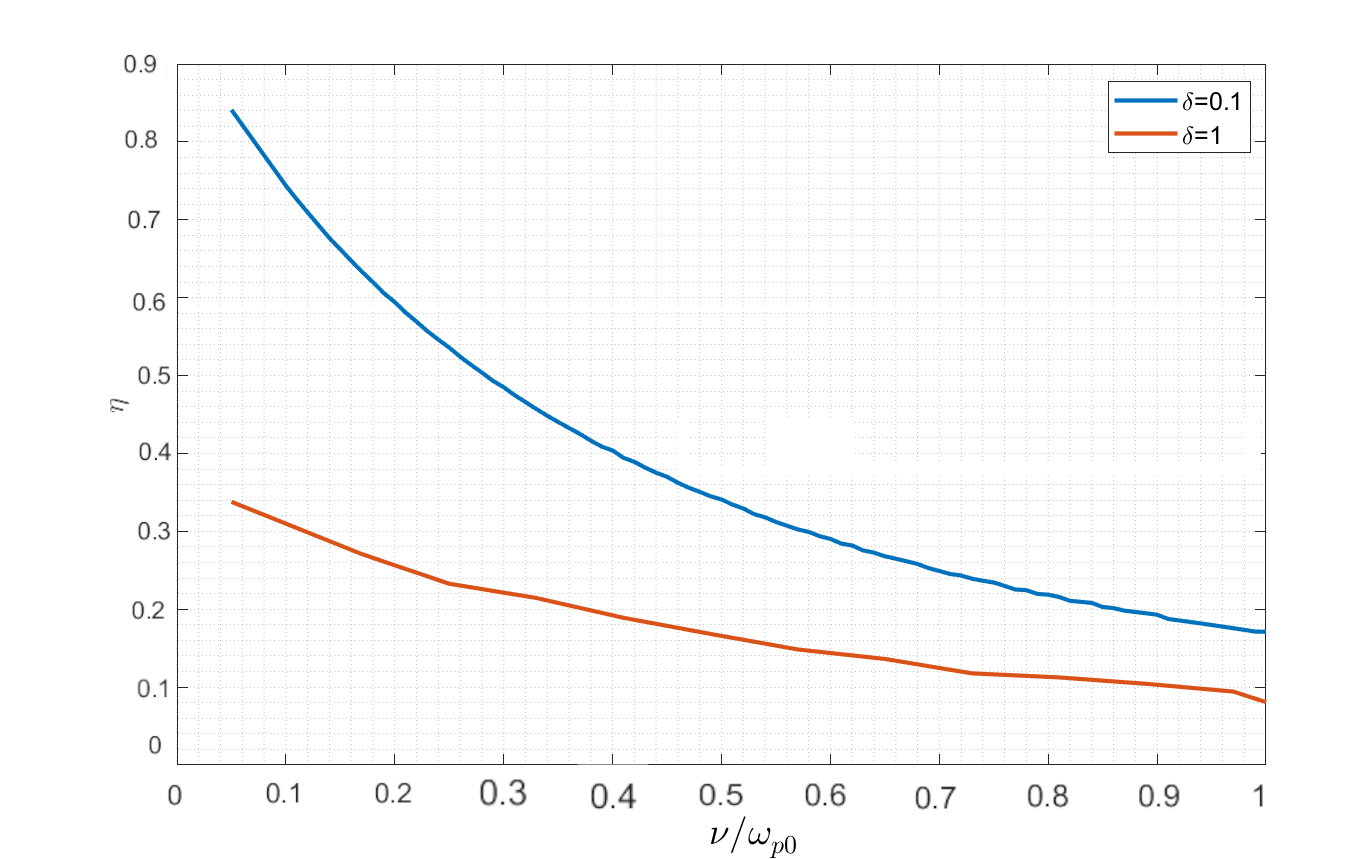
\includegraphics[width=1\linewidth]{pics/kpd_nu}
	\caption{Эффективность излучения в зависимости от частоты соударений $\nu/\omega_{p0}$ \\при разных размерах неоднородной области $\delta$.}
	\label{ris:kpd_nu}
\end{figure}

%% Generated using matlabfrag
% Version: v0.6.16
% Version Date: 04-Apr-2010
% Author: Zebb Prime
%
%% <text>
%
\providecommand\matlabtextA{\color[rgb]{0.150,0.150,0.150}\fontsize{1.320000e+01}{1.320000e+01}\selectfont\strut}%
\psfrag{015}[tc][tc]{\matlabtextA f}%
\psfrag{016}[bc][bc]{\matlabtextA Spectr}%
%
%% </text>
%
%% <xscale>
%
\providecommand\matlabtextB{\color[rgb]{0.150,0.150,0.150}\fontsize{12}{12}\selectfont\strut}%
\psfrag{000}[tc][tc]{\matlabtextB $\times10^{9}$}%
%
%% </xscale>
%
%% <xtick>
%
\def\matlabfragNegXTick{\mathord{\makebox[0pt][r]{$-$}}}
%
\psfrag{001}[ct][ct]{\matlabtextB $0$}%
\psfrag{002}[ct][ct]{\matlabtextB $0.5$}%
\psfrag{003}[ct][ct]{\matlabtextB $1$}%
\psfrag{004}[ct][ct]{\matlabtextB $1.5$}%
\psfrag{005}[ct][ct]{\matlabtextB $2$}%
\psfrag{006}[ct][ct]{\matlabtextB $2.5$}%
\psfrag{007}[ct][ct]{\matlabtextB $3$}%
%
%% </xtick>
%
%% <ytick>
%
\psfrag{008}[rc][rc]{\matlabtextB $0$}%
\psfrag{009}[rc][rc]{\matlabtextB $1$}%
\psfrag{010}[rc][rc]{\matlabtextB $2$}%
\psfrag{011}[rc][rc]{\matlabtextB $3$}%
\psfrag{012}[rc][rc]{\matlabtextB $4$}%
\psfrag{013}[rc][rc]{\matlabtextB $5$}%
\psfrag{014}[rc][rc]{\matlabtextB $6$}%
%
%% </ytick>

\section*{Заключение}

Разработана вычислительная программа на основе решения системы уравнений Максвелла в цилиндрической геометрии для расчета токов в плазме с быстро меняющейся плотностью и порождаемого ими электромагнитного излучение в плазме и окружающем пространстве.

На основе разработанной программы выполнены расчеты цилиндрического лазерно-плазменного излучателя электромагнитных (терагерцовых) волн и определена эффективность преобразования энергии,  запасенной в остаточных токах, в излученную энергию. Показано, что эффективность сильно падает с увеличением степени неоднородности плазмы. Найдены оптимальные значения радиуса плазменного цилиндра, отвечающие наибольшей эффективности преобразования энергии остаточных токов в электромагнитное излучение.

%\section*{Техника безопасности}

При пользовании средствами вычислительной техники и периферийным оборудованием каждый работник должен внимательно и осторожно обращаться с электропроводкой, приборами и аппаратами и всегда помнить, что пренебрежение правилами безопасности угрожает и здоровью, и жизни человека. Во избежание поражения электрическим током необходимо твердо знать и выполнять следующие правила безопасного пользования электроэнергией:

Во избежание повреждения изоляции проводов и возникновения коротких замыканий не разрешается:
\begin{itemize}
	\item вешать что-то на провода;
	\item закладывать провода и шнуры за газовые и водопроводные трубы, за батареи отопительной системы;
	\item выдергивать штепсельную вилку из розетки за шнур, усилие должно быть приложено к корпусу вилки.
\end{itemize}

Для исключения поражения электрическим током запрещается:
\begin{itemize}
	\item прикасаться к экрану и к тыльной стороне блоков компьютера; 
	\item работать на средствах вычислительной техники и периферийном оборудовании мокрыми руками; 
	\item класть на средства вычислительной техники и периферийном оборудовании посторонние предметы.
	\item ремонт электроаппаратуры производится только специалистами-техниками с соблюдением необходимых технических требований.
	\item недопустимо под напряжением проводить ремонт средств вычислительной техники и периферийного оборудования.	
\end{itemize}

Согласно медицинским нормам, работать за компьютером следует в течение двух часов, после чего необходимо делать перерыв.

\newpage
\section*{Приложение}

В ходе исполнения учебной практики также была проведена работа в преподавательской её части. Педагогическая (преподавательская) практика заключалась в принятии лабораторных работ на кафедре \textit{электродинамики} по теме \textbf{<<Исследование отражательного клистрона>>} у трёх пар студентов 3-го курса по направлению <<Специальные радиотехнические системы>>.  

В ходе прохождения преподавательской практики требовалось:
\begin{enumerate}
	\item Раздать студентам \textit{методические пособия} по работе;
	\item Принять \textit{допуск} у каждого студента отдельно;
	\item Проконсультировать студентов по вопросам выполнения \textit{практической части} работы;
	\item Принять отчеты о проделанной работе.
\end{enumerate}

Допуск к лабораторной работе принимался в виде личной беседы. Основные вопросы, на которые отвечали студенты, следующие:
\begin{itemize}
	\item Как устроен, из каких основных компонентов (составляющих) состоит отражательный клистрон?
	\item Каков принцип работы отражательного клистрона? В чем его основная функция?
	\item Каким образом происходит генерация СВЧ излучения?
	\item Что такое зоны генерации клистрона? Каков принцип их возникновения?
	\item Можно ли для возвращения электронного потока в резонатор клистрона использовать не постоянное электрическое, а постоянное магнитное поле?
\end{itemize}

После сдачи допуска группа(-ы) студентов выполняют экспериментальную практическую часть в соответствии с методическим пособием. При выполнении составляется протокол о проделанной работе, используя данные с которого, составляется итоговый отчет. Сдача отчета подразумевает личную беседу с вопросами, основанными на составленном отчете: проверяется подлинность измерений, точность и корректность их изображения в виде графиков/диаграмм/и т.д., а также оцениваются знания студентов по уже изученной работе.

\newpage
\printbibliography
\end{document}